\section{Method}

\subsection{Data Simulation}
\label{sec:data-simulation}
To train the phoneme recognition model, accurate labels are essential, mapping directly to the word being pronounced. Thus, we follow the TTS-based dysfluency simulation pipeline described in~\cite{zhou24eyolostutter}. First, we inject phonetic substitutions into each word from the text of the VCTK corpus~\cite{yamagishi2019cstr-vctk} based on a predefined set of common phoneme substitution pairs listed in Table. ~\ref{table-sub}, which include vowel-to-vowel and consonant-to-consonant substitutions respectively. Next, we input the modified IPA sequences into the VITS~\cite{kim2021conditional-vits} model to generate speech with phonetic errors. These resulting \textit{(speech, modified phoneme sequence, reference word)} pairs are used as training data for our phoneme recognition model.

\vspace{-5pt}
\begin{table}[h]
    \caption{Common CMU phoneme substitution pairs}
    \label{table-sub}
    \centering
    \setlength{\tabcolsep}{6pt} 
    \renewcommand{\arraystretch}{1.2} 
    \resizebox{8cm}{!}{
    \begin{tabular}{c c c | c c c c} 
     \toprule
    \multicolumn{3}{c|}{\textbf{Vowel}} & \multicolumn{4}{c}{\textbf{Consonant}} \\
    \hline
    \hline
    % \textipa{(a, i)} & \textipa{(æ, u)} & \textipa{(\char"0250, \char"026A)} & \textipa{(p, ɡ)} & \textipa{(t, ʒ)} & \textipa{(k, b)} & \textipa{(m, s)} \\
    % \textipa{(o, ɛ)} & \textipa{(ɔ, e)} & \textipa{(ʊ, ɜ)} & \textipa{(n, ʃ)} & \textipa{(ŋ, f)} & \textipa{(l, t)} & \textipa{(ɹ, d)} \\
    % \textipa{(ə, i)} & \textipa{(ɚ, o)} & \textipa{(ʌ, æ)} & \textipa{(w, k)} & \textipa{(θ, v)} & \textipa{(ð, z)} & \textipa{(ʃ, h)} \\
    (AA, IY) & (AE, UW) & (AA, IH) & (P, G) & (T, ZH) & (K, B) & (M, S) \\
    (OW, EH) & (AO, EH) & (UH, ER) & (N, SH) & (NG, F) & (L, T) & (R, D) \\
    (AH, IY) & (ER, OW) & (AH, AE) & (W, K) & (TH, V) & (DH, Z) & (SH, HH) \\
    \bottomrule
    \end{tabular}}
\end{table}



\vspace{-5pt}
\subsection{Phoneme Similarity Modeling} \label{sec:phn-similarity}
Unlike~\cite{lee2025dypcl} directly obtained the phoneme distance using PanPhon tool~\cite{mortensen-etal-2016-panphon}, we propose three methods for modeling phoneme similarity: heuristic-based, articulatory-based and Sylber-based methods. By incorporating perspectives from acoustics and syllables, these approaches more closely align with human pronunciation and auditory perception. We obtain a phoneme similarity matrix $S \in \mathbb{R}^{N \times N}$, where each value in the range $(0, 1)$, indicating the similarity between each pair of phonemes. $N$ represents the size of the phoneme dictionary.



\subsubsection{Heuristic-based}
Heuristic-based method calculates similarity by comparing phonemes based on eight features~\cite{anderson2018essentials}: vowel or consonant, vowel length, vowel height, vowel frontness, lip rounding, consonant type, place of articulation, and consonant voicing. Each feature is assigned a normalized weight, and the similarity score between pairs of phonemes is computed by summing the weights of matching feature values. In this study, the weights are set as follows: 0.2, 0.1, 0.15, 0.15, 0.1, 0.2, 0.2, and 0.1, respectively. The visualization of the phoneme similarity matrix is presented in Figure~\ref{fig:sim}.


\subsubsection{Articulatory-based} \label{sec:art-based}
We first construct a reference articulatory position for each phoneme using the VCTK corpus and an acoustic-to-articulatory inversion (AAI) model~\cite{cho2024jstsp}, employing a data-driven approach. Next, we compute the L2 distance between each pair of phonemes and apply min-max normalization to obtain the similarity scores.

\subsubsection{Sylber-based}
Human speech segmentation is natually syllabic~\cite{cho2024sylber}. We then utilize the Sylber~\cite{cho2024sylber} feature, as it offers a clean and robust syllabic structure. First, we fine-tune Sylber using a phoneme classification task with a single linear classifier layer, employing the VCTK corpus. Then, following a similar approach outlined in Sec.~\ref{sec:art-based}, we construct a reference feature for each phoneme and compute the similarity score.

Overall, the heuristic-based method stems from the perspective of phoneme classification and definition. Both the articulatory and Sylber-based methods are data-driven approaches: the former emphasizes the acoustic aspect, while the latter focuses more on the syllabic aspect.


\begin{figure}[t]
    \centering
    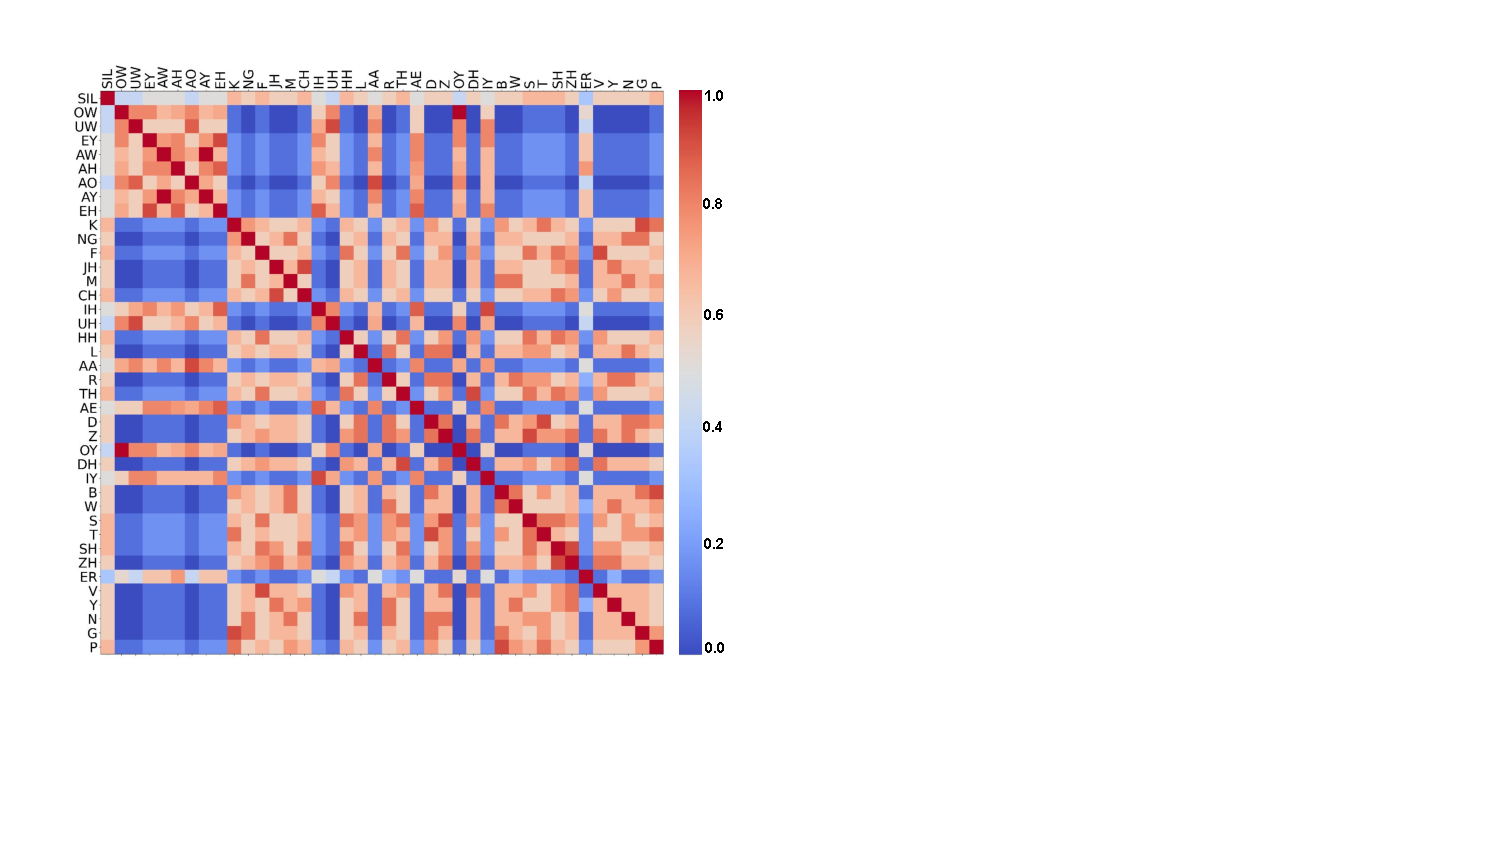
\includegraphics[height=6.8cm]{img/sim1.pdf}
    \caption{Heuristic-based phoneme similarity matrix}
    \label{fig:sim}
\end{figure}






\subsection{Verbatim Phoneme Recognition}
We adopt the speech feature extracted from WavLM~\cite{wavlm} to train a verbatim phoneme recognition model with multi-task learning and soft-training. 
The entire pipeline is illustrated in Figure~\ref{fig:pipeline}, and the model architecture and training objectives are described in the following sections.


\begin{figure*}[ht]
    \centering
    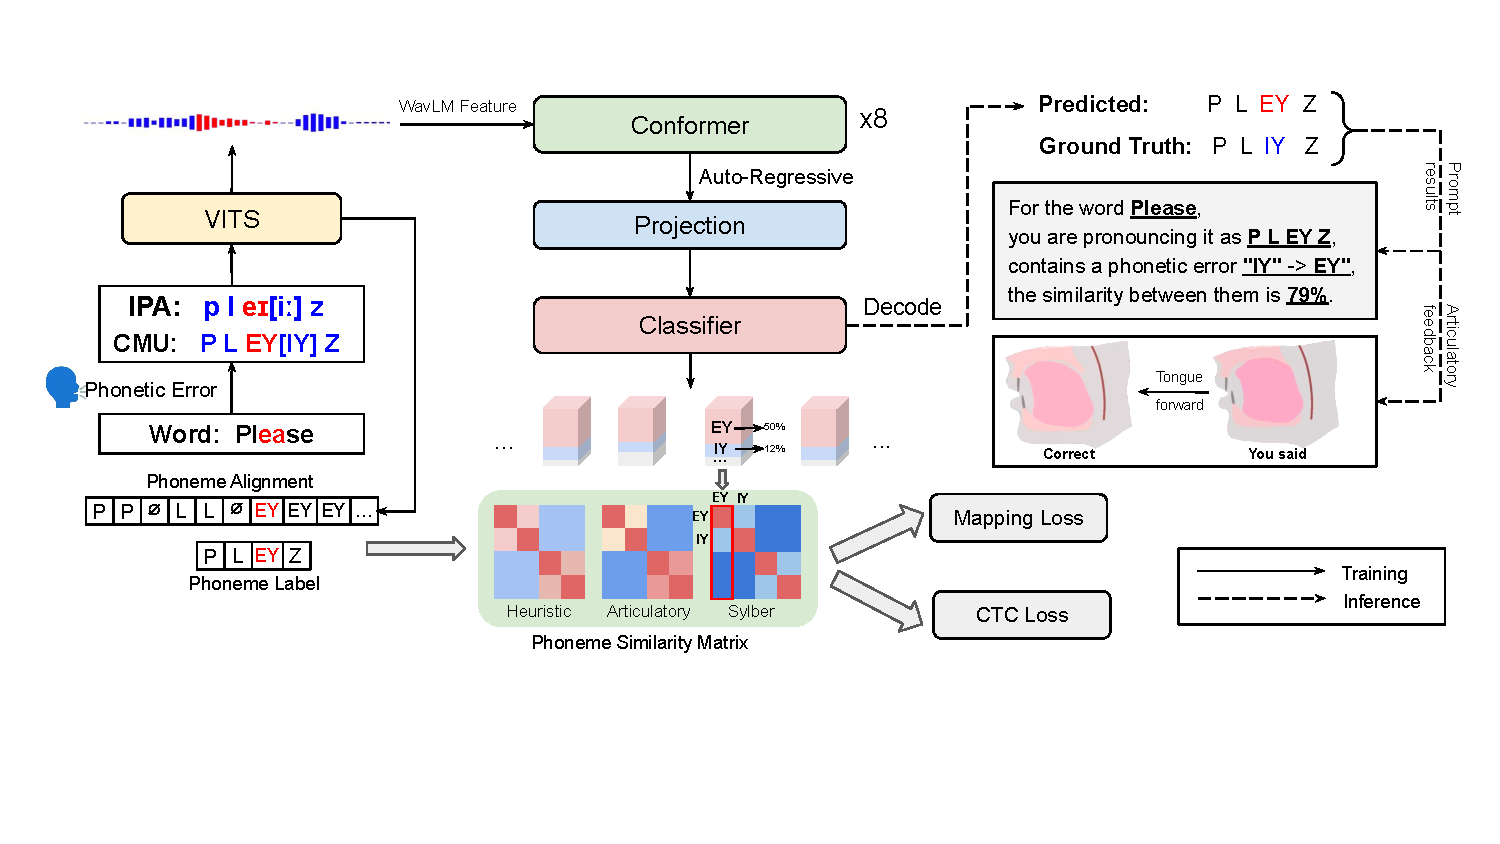
\includegraphics[width=16.5cm]{img/main.pdf}
    \caption{Pipeline of phoneme recognition and error detection: phonetic error of "IY" -> "EY" with a similarity score 79\% in the word "Please", and the articulatory feedback is moving the tongue towards the front of the mouth.}
    \label{fig:pipeline}
\end{figure*}



\subsubsection{Model}
The phoneme recognition model consists of a conformer~\cite{conformer} encoder, an autoregressive projection layer, and a linear classifier. This conformer encoder consists of 8 layers with 4 attention heads per layer. For the auto-regressive mechanism, For the autoregressive mechanism, at each timestep, the model combines the output features from the conformer encoder with the embedding of the previously predicted phoneme to predict the next phoneme, thereby effectively capturing the sequential dependencies in the data.



\subsubsection{Multi-task Learning and Soft-training}
We employ weighted loss-based multi-task training pipeline with two separate loss values: soft-CTC loss and soft-mapping loss. 
For the phoneme similarity matrix, each column(row) represents the similarity score of this phoneme and all other phonemes. We can treat this vector as a \textit{soft label} of this phoneme.
For soft-CTC loss, we utilize the target phoneme's soft label to weight the emission probability, thereby reducing the penalty for prediction errors between similar phonemes.
Traditional cross-entropy loss treats all phonemes as independent and ignores their similarities. Thus, in soft-mapping loss, we replace the one-hot encoded target with the target phoneme's soft label.
The complete loss is shown below:

\vspace{-5pt}
\begin{align} \label{equation:multi-loss}
\mathbb{L} &= \lambda_{ctc} \cdot L_{sCTC} + \lambda_{map} \cdot L_{smap} \notag \\
&= -\lambda_{ctc} \cdot \log \left( \sum_{z \in \mathcal{B}(y)} \prod_{t=1}^{T} \sum_{j=1}^{N} \hat{S}(z_t, j) \cdot p_t(j) \right) \notag \\
&\quad +\lambda_{map} \cdot \sum_{t=1}^{T} \sum_{j=1}^{N} (p_{t}(j) - \hat{S}(y_t,j))^2
\end{align}
Where $S$ denotes the normalized phoneme similarity matrix, $\mathcal{B}(y)$ denotes the set of all compatible alignments, $y$ is the target phoneme sequence, $p$ is model's output emission probability, and and $N$ is the phoneme dictionary size. In this work, we set $\lambda_{CTC}=0.8$, $\lambda_{map}=0.2$.



% \subsubsection{Contrastive Learning}

% \begin{align} \label{equation:contrasive}
%    \mathbb{L} = (\frac{1}{3}\sum^{(A,P,N)} L_{CTC} + L_{smap}) + \lambda \cdot L_{triplet}(a,\ p,\ n)
% \end{align}

% where $A$, $P$, and $N$ denote the anchor, positive,
% and negative audio samples, respectively, and $a$,
% $p$, and $n$ are the corresponding anchor, positive,
% and negative phonemes.